\subsection{/home/erik/git/dev/\+Lime\+S\+D\+R-\/\+U\+S\+B\+\_\+\+G\+W/ip/ddr2/ddr2\+\_\+phy\+\_\+report\+\_\+timing\+\_\+core.tcl File Reference}
\label{ddr2__phy__report__timing__core_8tcl}\index{/home/erik/git/dev/\+Lime\+S\+D\+R-\/\+U\+S\+B\+\_\+\+G\+W/ip/ddr2/ddr2\+\_\+phy\+\_\+report\+\_\+timing\+\_\+core.\+tcl@{/home/erik/git/dev/\+Lime\+S\+D\+R-\/\+U\+S\+B\+\_\+\+G\+W/ip/ddr2/ddr2\+\_\+phy\+\_\+report\+\_\+timing\+\_\+core.\+tcl}}


\subsubsection{Function Documentation}
\index{ddr2\+\_\+phy\+\_\+report\+\_\+timing\+\_\+core.\+tcl@{ddr2\+\_\+phy\+\_\+report\+\_\+timing\+\_\+core.\+tcl}!perform\+\_\+ac\+\_\+analyses@{perform\+\_\+ac\+\_\+analyses}}
\index{perform\+\_\+ac\+\_\+analyses@{perform\+\_\+ac\+\_\+analyses}!ddr2\+\_\+phy\+\_\+report\+\_\+timing\+\_\+core.\+tcl@{ddr2\+\_\+phy\+\_\+report\+\_\+timing\+\_\+core.\+tcl}}
\paragraph[{perform\+\_\+ac\+\_\+analysesopcs opcname pin\+\_\+array\+\_\+name timing\+\_\+parameters\+\_\+array\+\_\+name summary\+\_\+name I\+P\+\_\+name }]{\setlength{\rightskip}{0pt plus 5cm}perform\+\_\+ac\+\_\+analyses
\begin{DoxyParamCaption}
\item[{}]{opcs opcname pin\+\_\+array\+\_\+name timing\+\_\+parameters\+\_\+array\+\_\+name summary\+\_\+name I\+P\+\_\+name }
\end{DoxyParamCaption}
}\label{ddr2__phy__report__timing__core_8tcl_a36178bc38f9dfa158be9efe46fb96863}


Definition at line {\bf 1686} of file {\bf ddr2\+\_\+phy\+\_\+report\+\_\+timing\+\_\+core.\+tcl}.

\index{ddr2\+\_\+phy\+\_\+report\+\_\+timing\+\_\+core.\+tcl@{ddr2\+\_\+phy\+\_\+report\+\_\+timing\+\_\+core.\+tcl}!perform\+\_\+flexible\+\_\+read\+\_\+capture\+\_\+non\+\_\+dqs\+\_\+timing\+\_\+analysis@{perform\+\_\+flexible\+\_\+read\+\_\+capture\+\_\+non\+\_\+dqs\+\_\+timing\+\_\+analysis}}
\index{perform\+\_\+flexible\+\_\+read\+\_\+capture\+\_\+non\+\_\+dqs\+\_\+timing\+\_\+analysis@{perform\+\_\+flexible\+\_\+read\+\_\+capture\+\_\+non\+\_\+dqs\+\_\+timing\+\_\+analysis}!ddr2\+\_\+phy\+\_\+report\+\_\+timing\+\_\+core.\+tcl@{ddr2\+\_\+phy\+\_\+report\+\_\+timing\+\_\+core.\+tcl}}
\paragraph[{perform\+\_\+flexible\+\_\+read\+\_\+capture\+\_\+non\+\_\+dqs\+\_\+timing\+\_\+analysisopcs opcname pin\+\_\+array\+\_\+name timing\+\_\+parameters\+\_\+array\+\_\+name summary\+\_\+name M\+P\+\_\+name I\+P\+\_\+name board\+\_\+parameters\+\_\+name }]{\setlength{\rightskip}{0pt plus 5cm}perform\+\_\+flexible\+\_\+read\+\_\+capture\+\_\+non\+\_\+dqs\+\_\+timing\+\_\+analysis
\begin{DoxyParamCaption}
\item[{}]{opcs opcname pin\+\_\+array\+\_\+name timing\+\_\+parameters\+\_\+array\+\_\+name summary\+\_\+name M\+P\+\_\+name I\+P\+\_\+name board\+\_\+parameters\+\_\+name }
\end{DoxyParamCaption}
}\label{ddr2__phy__report__timing__core_8tcl_a238243d7aa214956c89aba6dc4bec4d2}


First get the min/max range of DQ and. 

clock signals. Can be a result of Now compute the margin from the ideal 

Definition at line {\bf 908} of file {\bf ddr2\+\_\+phy\+\_\+report\+\_\+timing\+\_\+core.\+tcl}.



References {\bf max\+\_\+in\+\_\+collection()}, and {\bf min\+\_\+in\+\_\+collection()}.



Here is the call graph for this function\+:\nopagebreak
\begin{figure}[H]
\begin{center}
\leavevmode
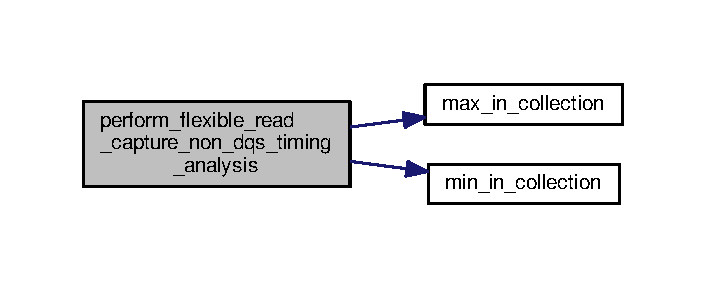
\includegraphics[width=339pt]{d8/d60/ddr2__phy__report__timing__core_8tcl_a238243d7aa214956c89aba6dc4bec4d2_cgraph}
\end{center}
\end{figure}


\index{ddr2\+\_\+phy\+\_\+report\+\_\+timing\+\_\+core.\+tcl@{ddr2\+\_\+phy\+\_\+report\+\_\+timing\+\_\+core.\+tcl}!perform\+\_\+flexible\+\_\+read\+\_\+capture\+\_\+timing\+\_\+analysis@{perform\+\_\+flexible\+\_\+read\+\_\+capture\+\_\+timing\+\_\+analysis}}
\index{perform\+\_\+flexible\+\_\+read\+\_\+capture\+\_\+timing\+\_\+analysis@{perform\+\_\+flexible\+\_\+read\+\_\+capture\+\_\+timing\+\_\+analysis}!ddr2\+\_\+phy\+\_\+report\+\_\+timing\+\_\+core.\+tcl@{ddr2\+\_\+phy\+\_\+report\+\_\+timing\+\_\+core.\+tcl}}
\paragraph[{perform\+\_\+flexible\+\_\+read\+\_\+capture\+\_\+timing\+\_\+analysisopcs opcname pin\+\_\+array\+\_\+name timing\+\_\+parameters\+\_\+array\+\_\+name summary\+\_\+name M\+P\+\_\+name I\+P\+\_\+name }]{\setlength{\rightskip}{0pt plus 5cm}perform\+\_\+flexible\+\_\+read\+\_\+capture\+\_\+timing\+\_\+analysis
\begin{DoxyParamCaption}
\item[{}]{opcs opcname pin\+\_\+array\+\_\+name timing\+\_\+parameters\+\_\+array\+\_\+name summary\+\_\+name M\+P\+\_\+name I\+P\+\_\+name }
\end{DoxyParamCaption}
}\label{ddr2__phy__report__timing__core_8tcl_a1bb76b7a3257aca559661a59bec8bf5c}


Read Timing Analysis \subparagraph*{}

Consider some post calibration effects on calibration 

Definition at line {\bf 564} of file {\bf ddr2\+\_\+phy\+\_\+report\+\_\+timing\+\_\+core.\+tcl}.



References {\bf format\+\_\+3dp()}, {\bf get\+\_\+colours()}, {\bf max\+\_\+in\+\_\+collection()}, {\bf min()}, {\bf min\+\_\+in\+\_\+collection()}, and {\bf min\+\_\+in\+\_\+collection\+\_\+from\+\_\+name()}.



Here is the call graph for this function\+:\nopagebreak
\begin{figure}[H]
\begin{center}
\leavevmode
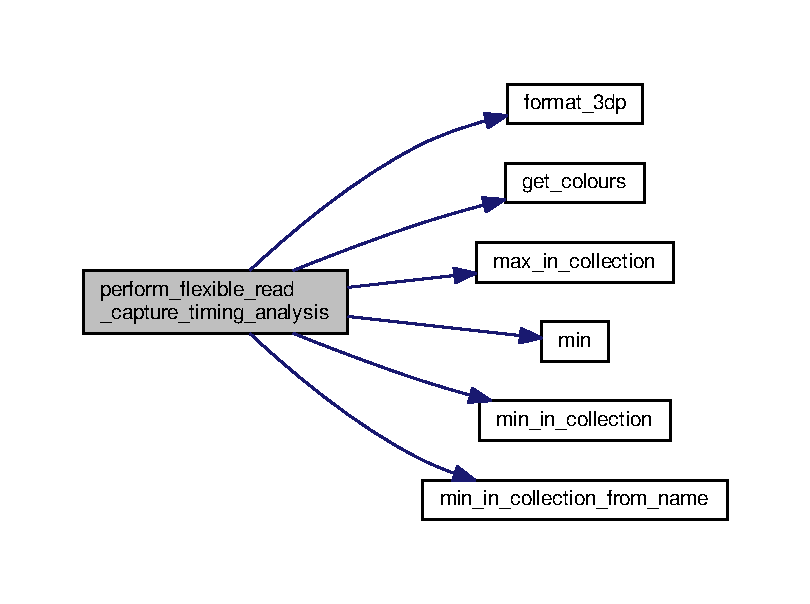
\includegraphics[width=350pt]{d8/d60/ddr2__phy__report__timing__core_8tcl_a1bb76b7a3257aca559661a59bec8bf5c_cgraph}
\end{center}
\end{figure}


\index{ddr2\+\_\+phy\+\_\+report\+\_\+timing\+\_\+core.\+tcl@{ddr2\+\_\+phy\+\_\+report\+\_\+timing\+\_\+core.\+tcl}!perform\+\_\+flexible\+\_\+resync\+\_\+timing\+\_\+analysis@{perform\+\_\+flexible\+\_\+resync\+\_\+timing\+\_\+analysis}}
\index{perform\+\_\+flexible\+\_\+resync\+\_\+timing\+\_\+analysis@{perform\+\_\+flexible\+\_\+resync\+\_\+timing\+\_\+analysis}!ddr2\+\_\+phy\+\_\+report\+\_\+timing\+\_\+core.\+tcl@{ddr2\+\_\+phy\+\_\+report\+\_\+timing\+\_\+core.\+tcl}}
\paragraph[{perform\+\_\+flexible\+\_\+resync\+\_\+timing\+\_\+analysisopcs opcname pin\+\_\+array\+\_\+name timing\+\_\+parameters\+\_\+array\+\_\+name summary\+\_\+name M\+P\+\_\+name I\+P\+\_\+name S\+S\+N\+\_\+name board\+\_\+parameters\+\_\+name }]{\setlength{\rightskip}{0pt plus 5cm}perform\+\_\+flexible\+\_\+resync\+\_\+timing\+\_\+analysis
\begin{DoxyParamCaption}
\item[{}]{opcs opcname pin\+\_\+array\+\_\+name timing\+\_\+parameters\+\_\+array\+\_\+name summary\+\_\+name M\+P\+\_\+name I\+P\+\_\+name S\+S\+N\+\_\+name board\+\_\+parameters\+\_\+name }
\end{DoxyParamCaption}
}\label{ddr2__phy__report__timing__core_8tcl_ae114685d4790b5292ccf8715b579333e}


Definition at line {\bf 1209} of file {\bf ddr2\+\_\+phy\+\_\+report\+\_\+timing\+\_\+core.\+tcl}.



References {\bf max\+\_\+in\+\_\+collection()}, and {\bf min\+\_\+in\+\_\+collection()}.



Here is the call graph for this function\+:\nopagebreak
\begin{figure}[H]
\begin{center}
\leavevmode
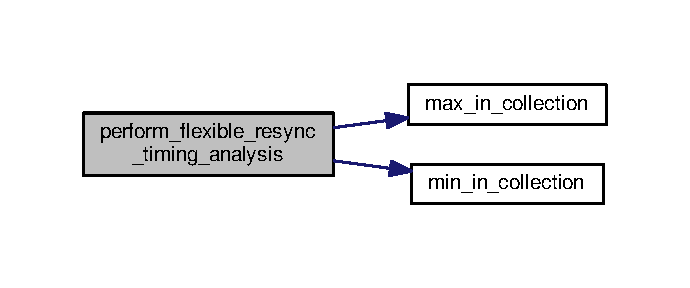
\includegraphics[width=331pt]{d8/d60/ddr2__phy__report__timing__core_8tcl_ae114685d4790b5292ccf8715b579333e_cgraph}
\end{center}
\end{figure}


\index{ddr2\+\_\+phy\+\_\+report\+\_\+timing\+\_\+core.\+tcl@{ddr2\+\_\+phy\+\_\+report\+\_\+timing\+\_\+core.\+tcl}!perform\+\_\+flexible\+\_\+write\+\_\+launch\+\_\+timing\+\_\+analysis@{perform\+\_\+flexible\+\_\+write\+\_\+launch\+\_\+timing\+\_\+analysis}}
\index{perform\+\_\+flexible\+\_\+write\+\_\+launch\+\_\+timing\+\_\+analysis@{perform\+\_\+flexible\+\_\+write\+\_\+launch\+\_\+timing\+\_\+analysis}!ddr2\+\_\+phy\+\_\+report\+\_\+timing\+\_\+core.\+tcl@{ddr2\+\_\+phy\+\_\+report\+\_\+timing\+\_\+core.\+tcl}}
\paragraph[{perform\+\_\+flexible\+\_\+write\+\_\+launch\+\_\+timing\+\_\+analysisopcs opcname pin\+\_\+array\+\_\+name timing\+\_\+parameters\+\_\+array\+\_\+name summary\+\_\+name M\+P\+\_\+name I\+P\+\_\+name }]{\setlength{\rightskip}{0pt plus 5cm}perform\+\_\+flexible\+\_\+write\+\_\+launch\+\_\+timing\+\_\+analysis
\begin{DoxyParamCaption}
\item[{}]{opcs opcname pin\+\_\+array\+\_\+name timing\+\_\+parameters\+\_\+array\+\_\+name summary\+\_\+name M\+P\+\_\+name I\+P\+\_\+name }
\end{DoxyParamCaption}
}\label{ddr2__phy__report__timing__core_8tcl_a2be65d48c3c91665784384ccd141d3ea}


Write Timing Analysis \subparagraph*{}

Consider some post calibration effects on calibration 

Definition at line {\bf 5} of file {\bf ddr2\+\_\+phy\+\_\+report\+\_\+timing\+\_\+core.\+tcl}.



References {\bf format\+\_\+3dp()}, {\bf get\+\_\+all\+\_\+dqs\+\_\+pins()}, {\bf get\+\_\+colours()}, {\bf get\+\_\+output\+\_\+clock\+\_\+id()}, {\bf max\+\_\+in\+\_\+collection()}, {\bf min()}, {\bf min\+\_\+in\+\_\+collection()}, and {\bf min\+\_\+in\+\_\+collection\+\_\+to\+\_\+name()}.



Here is the call graph for this function\+:\nopagebreak
\begin{figure}[H]
\begin{center}
\leavevmode
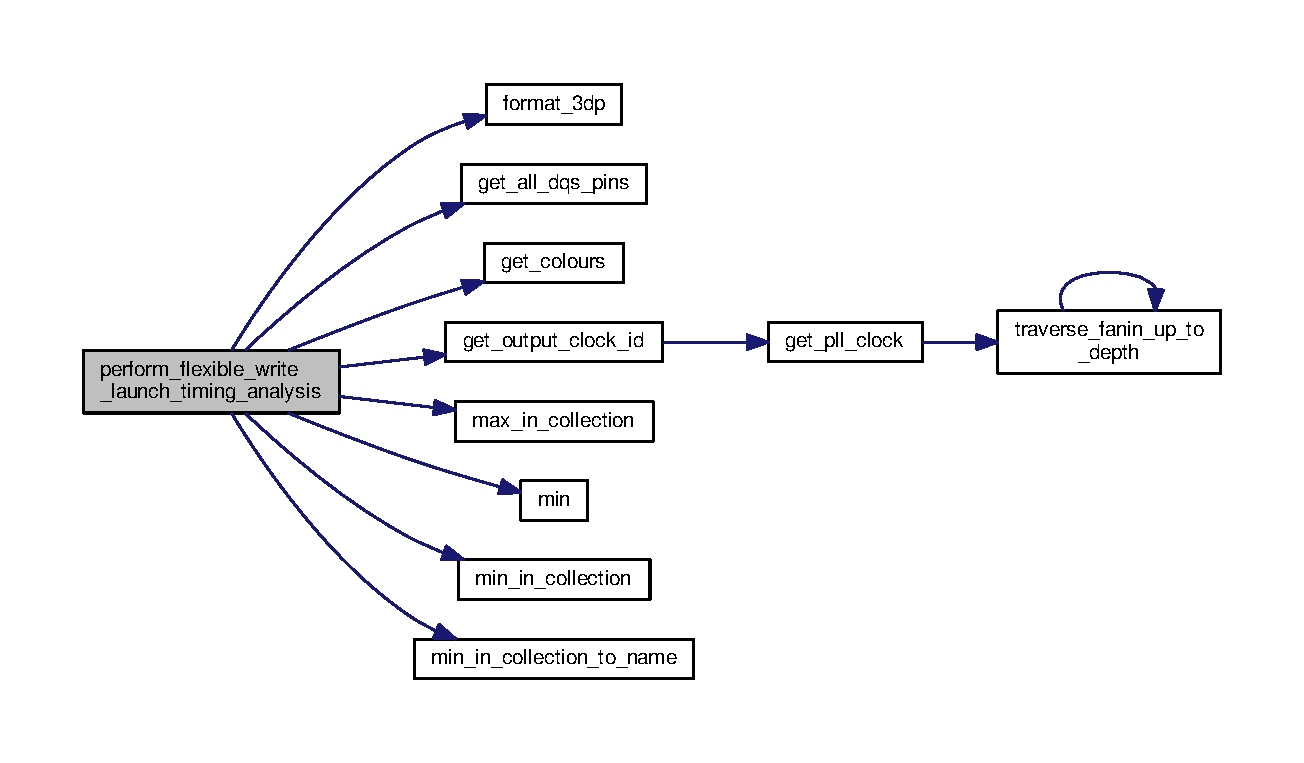
\includegraphics[width=350pt]{d8/d60/ddr2__phy__report__timing__core_8tcl_a2be65d48c3c91665784384ccd141d3ea_cgraph}
\end{center}
\end{figure}


\index{ddr2\+\_\+phy\+\_\+report\+\_\+timing\+\_\+core.\+tcl@{ddr2\+\_\+phy\+\_\+report\+\_\+timing\+\_\+core.\+tcl}!perform\+\_\+flexible\+\_\+write\+\_\+levelling\+\_\+timing\+\_\+analysis@{perform\+\_\+flexible\+\_\+write\+\_\+levelling\+\_\+timing\+\_\+analysis}}
\index{perform\+\_\+flexible\+\_\+write\+\_\+levelling\+\_\+timing\+\_\+analysis@{perform\+\_\+flexible\+\_\+write\+\_\+levelling\+\_\+timing\+\_\+analysis}!ddr2\+\_\+phy\+\_\+report\+\_\+timing\+\_\+core.\+tcl@{ddr2\+\_\+phy\+\_\+report\+\_\+timing\+\_\+core.\+tcl}}
\paragraph[{perform\+\_\+flexible\+\_\+write\+\_\+levelling\+\_\+timing\+\_\+analysisopcs opcname pin\+\_\+array\+\_\+name timing\+\_\+parameters\+\_\+array\+\_\+name summary\+\_\+name M\+P\+\_\+name I\+P\+\_\+name S\+S\+N\+\_\+name board\+\_\+parameters\+\_\+name I\+S\+I\+\_\+parameters\+\_\+name }]{\setlength{\rightskip}{0pt plus 5cm}perform\+\_\+flexible\+\_\+write\+\_\+levelling\+\_\+timing\+\_\+analysis
\begin{DoxyParamCaption}
\item[{}]{opcs opcname pin\+\_\+array\+\_\+name timing\+\_\+parameters\+\_\+array\+\_\+name summary\+\_\+name M\+P\+\_\+name I\+P\+\_\+name S\+S\+N\+\_\+name board\+\_\+parameters\+\_\+name I\+S\+I\+\_\+parameters\+\_\+name }
\end{DoxyParamCaption}
}\label{ddr2__phy__report__timing__core_8tcl_a3dbfc6d03d6eead0103af68731a5b203}


Definition at line {\bf 1433} of file {\bf ddr2\+\_\+phy\+\_\+report\+\_\+timing\+\_\+core.\+tcl}.

\index{ddr2\+\_\+phy\+\_\+report\+\_\+timing\+\_\+core.\+tcl@{ddr2\+\_\+phy\+\_\+report\+\_\+timing\+\_\+core.\+tcl}!perform\+\_\+macro\+\_\+read\+\_\+capture\+\_\+timing\+\_\+analysis@{perform\+\_\+macro\+\_\+read\+\_\+capture\+\_\+timing\+\_\+analysis}}
\index{perform\+\_\+macro\+\_\+read\+\_\+capture\+\_\+timing\+\_\+analysis@{perform\+\_\+macro\+\_\+read\+\_\+capture\+\_\+timing\+\_\+analysis}!ddr2\+\_\+phy\+\_\+report\+\_\+timing\+\_\+core.\+tcl@{ddr2\+\_\+phy\+\_\+report\+\_\+timing\+\_\+core.\+tcl}}
\paragraph[{perform\+\_\+macro\+\_\+read\+\_\+capture\+\_\+timing\+\_\+analysisopcs opcname pin\+\_\+array\+\_\+name timing\+\_\+parameters\+\_\+array\+\_\+name summary\+\_\+name I\+P\+\_\+name }]{\setlength{\rightskip}{0pt plus 5cm}perform\+\_\+macro\+\_\+read\+\_\+capture\+\_\+timing\+\_\+analysis
\begin{DoxyParamCaption}
\item[{}]{opcs opcname pin\+\_\+array\+\_\+name timing\+\_\+parameters\+\_\+array\+\_\+name summary\+\_\+name I\+P\+\_\+name }
\end{DoxyParamCaption}
}\label{ddr2__phy__report__timing__core_8tcl_a8ce9952997f1cd6cd92a056dfa2fe987}


Definition at line {\bf 1020} of file {\bf ddr2\+\_\+phy\+\_\+report\+\_\+timing\+\_\+core.\+tcl}.



References {\bf get\+\_\+all\+\_\+dqs\+\_\+pins()}, {\bf get\+\_\+tsw()}, and {\bf round\+\_\+3dp()}.



Here is the call graph for this function\+:\nopagebreak
\begin{figure}[H]
\begin{center}
\leavevmode
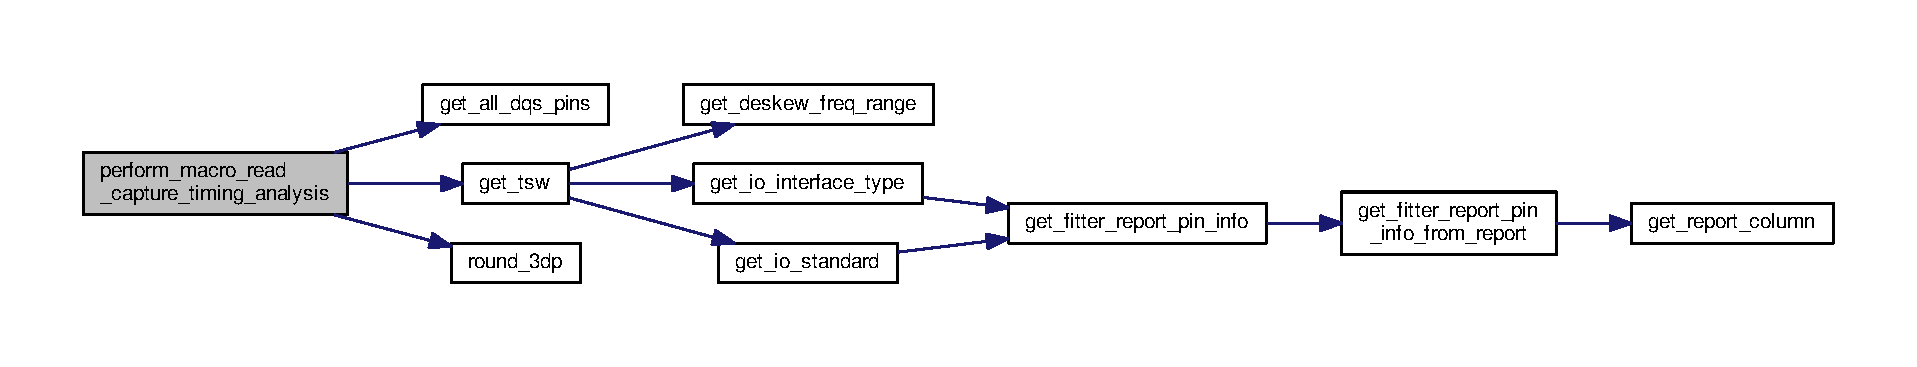
\includegraphics[width=350pt]{d8/d60/ddr2__phy__report__timing__core_8tcl_a8ce9952997f1cd6cd92a056dfa2fe987_cgraph}
\end{center}
\end{figure}


\index{ddr2\+\_\+phy\+\_\+report\+\_\+timing\+\_\+core.\+tcl@{ddr2\+\_\+phy\+\_\+report\+\_\+timing\+\_\+core.\+tcl}!perform\+\_\+macro\+\_\+resync\+\_\+timing\+\_\+analysis@{perform\+\_\+macro\+\_\+resync\+\_\+timing\+\_\+analysis}}
\index{perform\+\_\+macro\+\_\+resync\+\_\+timing\+\_\+analysis@{perform\+\_\+macro\+\_\+resync\+\_\+timing\+\_\+analysis}!ddr2\+\_\+phy\+\_\+report\+\_\+timing\+\_\+core.\+tcl@{ddr2\+\_\+phy\+\_\+report\+\_\+timing\+\_\+core.\+tcl}}
\paragraph[{perform\+\_\+macro\+\_\+resync\+\_\+timing\+\_\+analysisopcs opcname pin\+\_\+array\+\_\+name timing\+\_\+parameters\+\_\+array\+\_\+name summary\+\_\+name M\+P\+\_\+name I\+P\+\_\+name board\+\_\+parameters\+\_\+name }]{\setlength{\rightskip}{0pt plus 5cm}perform\+\_\+macro\+\_\+resync\+\_\+timing\+\_\+analysis
\begin{DoxyParamCaption}
\item[{}]{opcs opcname pin\+\_\+array\+\_\+name timing\+\_\+parameters\+\_\+array\+\_\+name summary\+\_\+name M\+P\+\_\+name I\+P\+\_\+name board\+\_\+parameters\+\_\+name }
\end{DoxyParamCaption}
}\label{ddr2__phy__report__timing__core_8tcl_a8f3ed42d5a657b1c8125d89ba9d397df}


Calibrated Path Analysis \subparagraph*{}



Definition at line {\bf 1100} of file {\bf ddr2\+\_\+phy\+\_\+report\+\_\+timing\+\_\+core.\+tcl}.



References {\bf max\+\_\+in\+\_\+collection()}, {\bf min\+\_\+in\+\_\+collection()}, and {\bf round\+\_\+3dp()}.



Here is the call graph for this function\+:\nopagebreak
\begin{figure}[H]
\begin{center}
\leavevmode
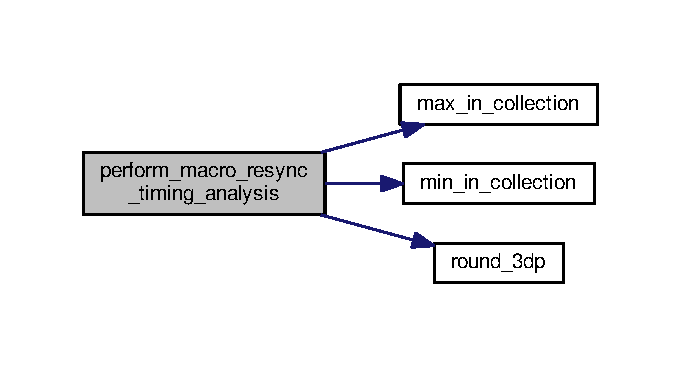
\includegraphics[width=327pt]{d8/d60/ddr2__phy__report__timing__core_8tcl_a8f3ed42d5a657b1c8125d89ba9d397df_cgraph}
\end{center}
\end{figure}


\index{ddr2\+\_\+phy\+\_\+report\+\_\+timing\+\_\+core.\+tcl@{ddr2\+\_\+phy\+\_\+report\+\_\+timing\+\_\+core.\+tcl}!perform\+\_\+macro\+\_\+write\+\_\+launch\+\_\+timing\+\_\+analysis@{perform\+\_\+macro\+\_\+write\+\_\+launch\+\_\+timing\+\_\+analysis}}
\index{perform\+\_\+macro\+\_\+write\+\_\+launch\+\_\+timing\+\_\+analysis@{perform\+\_\+macro\+\_\+write\+\_\+launch\+\_\+timing\+\_\+analysis}!ddr2\+\_\+phy\+\_\+report\+\_\+timing\+\_\+core.\+tcl@{ddr2\+\_\+phy\+\_\+report\+\_\+timing\+\_\+core.\+tcl}}
\paragraph[{perform\+\_\+macro\+\_\+write\+\_\+launch\+\_\+timing\+\_\+analysisopcs opcname pin\+\_\+array\+\_\+name timing\+\_\+parameters\+\_\+array\+\_\+name summary\+\_\+name I\+P\+\_\+name I\+S\+I\+\_\+name }]{\setlength{\rightskip}{0pt plus 5cm}perform\+\_\+macro\+\_\+write\+\_\+launch\+\_\+timing\+\_\+analysis
\begin{DoxyParamCaption}
\item[{}]{opcs opcname pin\+\_\+array\+\_\+name timing\+\_\+parameters\+\_\+array\+\_\+name summary\+\_\+name I\+P\+\_\+name I\+S\+I\+\_\+name }
\end{DoxyParamCaption}
}\label{ddr2__phy__report__timing__core_8tcl_a0b0f4f4dcf34d4e7f3b26d257f17589b}


Definition at line {\bf 478} of file {\bf ddr2\+\_\+phy\+\_\+report\+\_\+timing\+\_\+core.\+tcl}.



References {\bf get\+\_\+all\+\_\+dq\+\_\+pins()}, {\bf get\+\_\+all\+\_\+dqs\+\_\+pins()}, {\bf get\+\_\+output\+\_\+clock\+\_\+id()}, {\bf get\+\_\+tccs()}, {\bf round\+\_\+3dp()}, and {\bf sett\+\_\+collection()}.



Here is the call graph for this function\+:\nopagebreak
\begin{figure}[H]
\begin{center}
\leavevmode
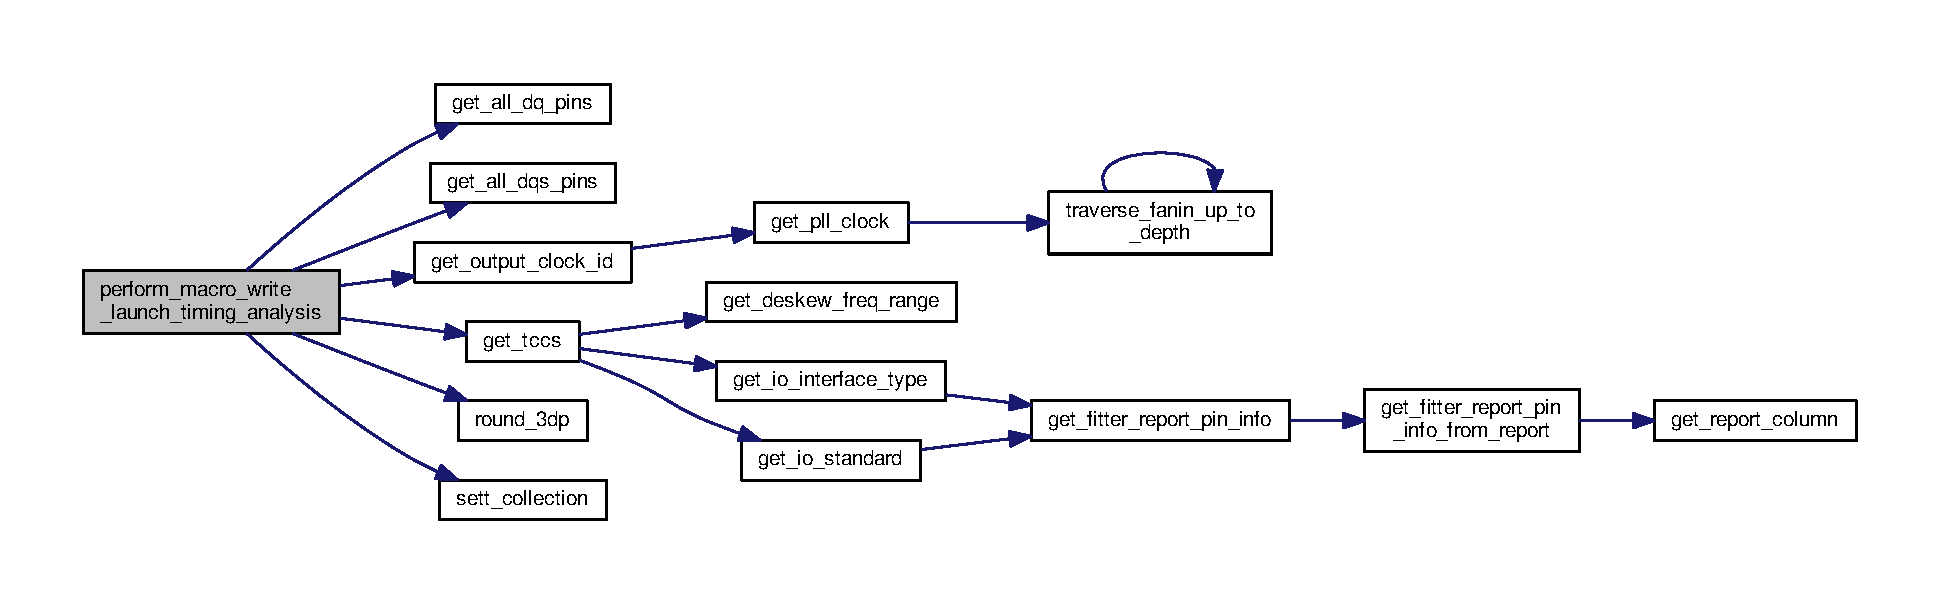
\includegraphics[width=350pt]{d8/d60/ddr2__phy__report__timing__core_8tcl_a0b0f4f4dcf34d4e7f3b26d257f17589b_cgraph}
\end{center}
\end{figure}


\index{ddr2\+\_\+phy\+\_\+report\+\_\+timing\+\_\+core.\+tcl@{ddr2\+\_\+phy\+\_\+report\+\_\+timing\+\_\+core.\+tcl}!perform\+\_\+macro\+\_\+write\+\_\+levelling\+\_\+timing\+\_\+analysis@{perform\+\_\+macro\+\_\+write\+\_\+levelling\+\_\+timing\+\_\+analysis}}
\index{perform\+\_\+macro\+\_\+write\+\_\+levelling\+\_\+timing\+\_\+analysis@{perform\+\_\+macro\+\_\+write\+\_\+levelling\+\_\+timing\+\_\+analysis}!ddr2\+\_\+phy\+\_\+report\+\_\+timing\+\_\+core.\+tcl@{ddr2\+\_\+phy\+\_\+report\+\_\+timing\+\_\+core.\+tcl}}
\paragraph[{perform\+\_\+macro\+\_\+write\+\_\+levelling\+\_\+timing\+\_\+analysisopcs opcname pin\+\_\+array\+\_\+name timing\+\_\+parameters\+\_\+array\+\_\+name summary\+\_\+name M\+P\+\_\+name I\+P\+\_\+name board\+\_\+parameters\+\_\+name I\+S\+I\+\_\+parameters\+\_\+name }]{\setlength{\rightskip}{0pt plus 5cm}perform\+\_\+macro\+\_\+write\+\_\+levelling\+\_\+timing\+\_\+analysis
\begin{DoxyParamCaption}
\item[{}]{opcs opcname pin\+\_\+array\+\_\+name timing\+\_\+parameters\+\_\+array\+\_\+name summary\+\_\+name M\+P\+\_\+name I\+P\+\_\+name board\+\_\+parameters\+\_\+name I\+S\+I\+\_\+parameters\+\_\+name }
\end{DoxyParamCaption}
}\label{ddr2__phy__report__timing__core_8tcl_aa84476501a380c88accbe9a3cf639fb7}


Definition at line {\bf 1364} of file {\bf ddr2\+\_\+phy\+\_\+report\+\_\+timing\+\_\+core.\+tcl}.



References {\bf round\+\_\+3dp()}.



Here is the call graph for this function\+:\nopagebreak
\begin{figure}[H]
\begin{center}
\leavevmode
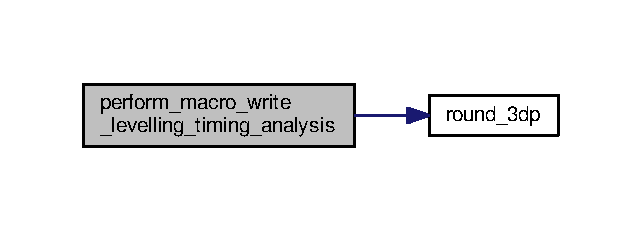
\includegraphics[width=308pt]{d8/d60/ddr2__phy__report__timing__core_8tcl_aa84476501a380c88accbe9a3cf639fb7_cgraph}
\end{center}
\end{figure}


\index{ddr2\+\_\+phy\+\_\+report\+\_\+timing\+\_\+core.\+tcl@{ddr2\+\_\+phy\+\_\+report\+\_\+timing\+\_\+core.\+tcl}!perform\+\_\+phy\+\_\+analyses@{perform\+\_\+phy\+\_\+analyses}}
\index{perform\+\_\+phy\+\_\+analyses@{perform\+\_\+phy\+\_\+analyses}!ddr2\+\_\+phy\+\_\+report\+\_\+timing\+\_\+core.\+tcl@{ddr2\+\_\+phy\+\_\+report\+\_\+timing\+\_\+core.\+tcl}}
\paragraph[{perform\+\_\+phy\+\_\+analysesopcs opcname pin\+\_\+array\+\_\+name timing\+\_\+parameters\+\_\+array\+\_\+name summary\+\_\+name I\+P\+\_\+name }]{\setlength{\rightskip}{0pt plus 5cm}perform\+\_\+phy\+\_\+analyses
\begin{DoxyParamCaption}
\item[{}]{opcs opcname pin\+\_\+array\+\_\+name timing\+\_\+parameters\+\_\+array\+\_\+name summary\+\_\+name I\+P\+\_\+name }
\end{DoxyParamCaption}
}\label{ddr2__phy__report__timing__core_8tcl_aa4ea4c079f8983b5094c7f21de6ac9ac}


Other Timing Analysis \subparagraph*{}



Definition at line {\bf 1616} of file {\bf ddr2\+\_\+phy\+\_\+report\+\_\+timing\+\_\+core.\+tcl}.



References {\bf min()}.



Here is the call graph for this function\+:\nopagebreak
\begin{figure}[H]
\begin{center}
\leavevmode
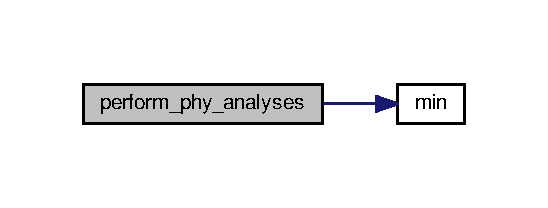
\includegraphics[width=263pt]{d8/d60/ddr2__phy__report__timing__core_8tcl_aa4ea4c079f8983b5094c7f21de6ac9ac_cgraph}
\end{center}
\end{figure}


